\documentclass[10pt,a4paper,twoside]{article}
% The following LaTeX packages must be installed on your machine: amsmath, authblk, bm, booktabs, caption, dcolumn, fancyhdr, geometry, graphicx, hyperref, latexsym, natbib

% Please make sure that spp.dat (supplied with this template) is in your working directory or path
\input{spp.dat}
\usepackage{multicol}
\usepackage{multirow}
\usepackage{xparse}
\usepackage{physics}
\usepackage{xcolor}

\newcommand{\snr}{\left(\dfrac{S}{N}\right)^2}
\newcommand{\dephase}{\exp(i\psi_{\text{env}})}


%  Editorial staff will uncomment the next line
% \providecommand{\artnum}[0]{XX-XX}
% \renewcommand{\articlenum}[0]{SPP-\the\year-\artnum-}

\begin{document}

%--------------------------------------------------
%  Fill in the paper's title in Sentence case
%  Titles beginning with articles (A, An, The) are discouraged
%--------------------------------------------------
\title{\TitleFont Probing the parameter constraints on astrophysical environments of IMRI and EMRI binaries with LISA}


%--------------------------------------------------
% For TWO authors with the same affiliation please use this block
% Or Please use the other author block templates
%--------------------------------------------------
\author[*\negthickspace]{Marco Immanuel B.~Rivera}
\author[ ]{Reinabelle C.~Reyes
\lastauthorsep}
\affil[ ]{National Institute of Physics, University of the Philippines, Diliman, Quezon City 1101, Philippines}
\affil[*]{\corremail{mrivera@nip.upd.edu.ph} }

%--------------------------------------------------
%  For three or more authors with the same affiliation please use this block
%--------------------------------------------------

% \author[*]{Author M.~Surname\authorsep}
% \author[ ]{Bauthor D.~Surname~Jr.\authorsep}
% \author[ ]{Cauthor D.~Surname~III\lastauthorsep}
% \affil[ ]{Department of Science, XXX University, Country}
% \affil[*]{\corremail{amsurname@university.edu} }

%--------------------------------------------------
%  For authors with different affiliations please use the following block
%--------------------------------------------------
% \author[1*]{Author M.~Surname\authorsep}
% \author[2]{Bauthor D.~Surname~Jr.\authorsep}
% \author[1,2]{Coauthor G.~Surname~III\authorsep}
% % !!! Please take note that the last author separation is \lastauthorsep instead of \authorsep
% \author[3]{Dauthor G.~Surname\lastauthorsep}
% \affil[1]{Department of Physics, DD University, Country}
% \affil[2]{Department of Science, XX University, Country}
% \affil[3]{Physics Institute, Country}
% \affil[*]{\corremail{amsurname@university.edu} }


\begin{abstract}
\noindent
%--------------------------------------------------
% Include abstract and keywords here
%--------------------------------------------------
The future space-borne Laser Interferometer Space Antenna (LISA) would allow detection of intermediate (IMRI) and extreme mass ratio inspirals (EMRI) via their gravitational wave (GW) emission. However, these binaries may live in nontrivial astrophysical environments, affecting their GW emission and thereby complicating detection and parameter estimation. By using Fisher matrix analysis, we calculate the uncertainties in the environmental density of inspirals with different mass ratios. We study several environmental effects affecting GW emission --- namely, gravitational pull, collisionless accretion, and gravitational drag --- and find a log-log relationship between the uncertainties and the primary mass of the binary. By using overlap analysis, we also get the signal-to-noise ratios (SNR) of the difference between a vacuum and an environmentally-modified waveform. We find that the dephasing brought about by environmental effects may be detectable within LISA's 4-year mission lifetime, especially for EMRIs.


\keywords{gravitational waves, LISA, Fisher matrix analysis, overlap analysis}

\end{abstract}

\maketitle
\thispagestyle{titlestyle}


%--------------------------------------------------
% the main text of your paper begins here
%--------------------------------------------------
\section{Introduction}\label{sec:intro}
%The future space-based Laser Interferometer Space Antenna (LISA) would open a new window in the gravitational wave (GW) spectrum \cite{amaroseoane2017lisa}. From the most recent model \cite{Robson2019} of its noise power spectral density (PSD), we expect GW detections in the range $[10^{-5}, 1]$ Hz. In this range, it is speculated that most sources would comprise of massive black hole binaries (MBHB) and extreme mass ratio inspirals (EMRI) \cite{Moore2015}.

%\textit{Context.} 
Astrophysical environments of compact object binaries may be probed by gravitational wave (GW) detectors such as the planned Laser Interferometer Space Antenna (LISA) \cite{barausse2014}. Previous work has shown that including environmental effects in the waveform --- namely gravitational pull, collisionless accretion, and gravitational drag (without dephasing from dynamical friction) --- would allow LISA to constrain the surrounding (constant) medium's density by up to $10^{-7} ~\text{kg}/\text{m}^3$, $10^{-13} ~\text{kg}/\text{m}^3$, and $10^{-22} ~\text{kg}/\text{m}^3$, respectively, for extreme mass ratio inspirals (EMRI) with mass ratio $q \equiv m_1/m_2 = 10^4$ \cite{Cardoso2020}. These values were calculated from the covariance matrix, which is the inverse of the Fisher information matrix in the limit of high signal-to-noise ratio (SNR). This Fisher information analysis has been extensively used in gravitational-wave astronomy to determine if planned detectors can accurately extract information from their specified targets \cite{Vallisneri2008}. 

%\textit{Content.} 
In this paper, we extend Cardoso and Maselli's analysis \cite{Cardoso2020} to binaries of varying mass ratios to see how the uncertainties depend on the primary mass of the binary. In effect, we are studying the manifold space of a waveform with dephasing from environmental effects. Since this space consists of many dimensions, we set constant some parameters such as the secondary mass ($m_2 = 10 ~M_{\odot}$), primary spin ($\chi_1 = 0.8$), secondary spin ($\chi_2 = 0.5$), and the luminosity distance of the binary ($d_L = 1$ Gpc) for simplicity. Here, $\chi_i = (c/G) S/m_i^2$ is the dimensionless spin angular momentum of the $i$th compact object \cite{ligo2017basic}. In particular, we look for trends in the uncertainty of the surrounding medium's density over a range of primary masses for several environmental effects. Furthermore, using overlap analysis, we determine if given the same dephasing factors, the perturbation between the vacuum and dephased waveforms would be significant for LISA. 

%We use the overlap analysis that involves the use of the overlap integral as seen in equation (7.46) of Maggiore \cite{maggiore2008gravitational}.

\section{Methodology}\label{sec:metho}
\subsection{Setup}
Following Cardoso and Maselli \cite{Cardoso2020}, we simulated several inspiralling quasi-circular compact binaries living in an astrophysical environment of constant density $\rho_0$. We then constructed frequency-domain vacuum waveforms within the stationary phase approximation (SPA) for these binaries, given by $\tilde{h}(f) = \mathcal{A}(f) e^{i\Psi(f)}$. Since we are working exclusively in the LISA frequency spectrum, we restrict our attention to black hole-black hole (BH-BH) binaries: in particular, intermediate (with $q \in [10^1, 10^3]$) and extreme (with $q \in [10^4, 10^5]$) mass ratio inspirals. We created a phenomenological inspiral-merger-ringdown (IMRPhenomB) waveform \cite{Ajith2011} for the GW phase $\Psi$ of a BH-BH binary with nonprecessing spins. We also adapted Berti et.~al's ``restricted post-Newtonian approximation" \cite{Berti2005} for the amplitude $\mathcal{A}$. 

To construct the environmentally-modified waveform, we multiplied the dephasing factor $\dephase = \exp (i\psi_{\text{GR}} \delta_{\psi_{\text{env}}})$ to the vacuum IMRPhenomB waveform. Here $\psi_{\text{GR}} = 3/128 (\mathcal{M} \pi f)^{-5/3}$ is the leading term in the PN expansion of the phase, $\mathcal{M} = M \eta^{3/5}$ is the chirp mass of the binary, $M \equiv m_1 + m_2$ is the total mass of the binary, $\eta \equiv (m_1 m_2)/M^2$ is the symmetric mass ratio, and $f$ is the GW frequency. The dephasing factors depend on the type of environmental effect considered; we use the following $\delta_{\psi_{\text{env}}}$ for a surrounding medium of constant density $\rho_0$: $\delta_{\psi_{\text{pull}}}(f) = f^{-2} \rho_0$, $\delta_{\psi_{\text{drag}}}(f) = -\eta^{-3} (1-3\eta) \pi^{-11/3} M^{-5/3} f^{-11/3} \rho_0$, and $\delta_{\psi_{\text{collisionless}}}(f) = -\eta^{-1}\pi^{-3} M^{-1} f^{-3} \rho_0$ \cite{Cardoso2020}. Here, ``pull" stands for the gravitational pull of the surrounding medium inside the orbital radius (centered at the binary's center of mass), ``drag" stands for the gravitational drag (without dephasing from dynamical friction) from the surrounding medium, and ``collisionless" stands for the collisionless accretion of the surrounding medium onto the central BH. All these factors depend on $\rho_0$ linearly. For the purpose of this analysis, these effects were considered independently of one another even though they might occur together in astrophysical environments.

\subsection{Fisher matrix calculation}\label{methoFisher} 
We calculate the Fisher matrix elements $\Gamma_{ij}$ as the overlap integral $\mathcal{O}$ \cite{maggiore2008gravitational} between the derivatives of the modified strain with respect to the relevant waveform parameters $\theta_i$, hereby listed with their fiducial values: $\{\ln \mathcal{M}/M_{\odot}, \ln \eta, \tau_c = 0, \phi_c = -\pi/4, \chi_{\text{eff}}, \rho_0 = 0 \}$. Here, $\tau_c$ represents the time at coalescence, $\phi_c$ the phase at coalescence, and $\chi_{\text{eff}} = (\chi_1 m_1 + \chi_2 m_2)/M$ the effective spin parameter. Explicitly,

\begin{equation}
    \Gamma_{ij} = \mathcal{O}\left(\dfrac{\partial \tilde{h}}{\partial \theta_i} \Bigg\rvert \dfrac{\partial \tilde{h}}{\partial \theta_j} \right) = 4 \Re \int_{f_{\text{min}}}^{f_{\text{max}}} \dfrac{df}{S_n(f)} \dfrac{\partial \tilde{h}}{\partial \theta_i} \left(\dfrac{\partial \tilde{h}}{\partial \theta_j}\right)^*,
\end{equation}

\noindent where Re denotes taking the real part, $^*$ denotes conjugation, and $S_n(f)$ is the power spectral density (PSD) of LISA, which has its latest semi-analytical expression provided in \cite{Robson2019}. The limits of integration are chosen such that the lower bound may be dependent on the time of observation $T_{\text{obs}}$ \cite{Berti2005}, while the upper bound may be dependent on $f_1$: the inspiral-merger transition frequency from Ajith et.~al's semi-analytical IMRPhenomB model \cite{Ajith2011}. They are given by

\begin{align}
f_{\text{min}} &= \max \left[10^{-5}, ~4.149 \times 10^{-5} \left(\dfrac{\mathcal{M}}{10^6 M_{\odot}}\right)^{-5/8} \left(\dfrac{T_{\text{obs}}}{1 \text{yr}}\right)^{-3/8} \right] ~\text{Hz}, \quad \text{and} \\
f_{\text{max}} &= \min \left[1, f_1\right] ~\text{Hz}. 
\end{align}

For these calculations, we set $T_{\text{obs}} = 4$ years. From $\Gamma_{ij}$, we can calculate the standard deviation $\sigma^{i}$ by inverting the Fisher matrix to get the covariance matrix $\Sigma^{ij} = (\Gamma^{-1})^{ij}$ and getting the square root of the diagonals: $\sigma^{i} = \sqrt{\Sigma^{ii}}$ \cite{maggiore2008gravitational, Vallisneri2008}.

\subsection{Signal-to-noise ratio (SNR) of the waveform difference}
To get the SNR of the waveform difference, we use the expression for the SNR with the Wiener filter already applied \cite{maggiore2008gravitational, Kocsis2011}:

\begin{align}
    \snr &= \mathcal{O}(\tilde{h}|\tilde{h}) = 4 \Re \int_{f_{\text{min}}}^{f_{\text{max}}} \dfrac{|\tilde{h}(f)|^2}{S_n(f)} df.
\end{align}

\noindent We then make the SNR a function of $T_{\text{obs}}$ to see how it accumulates over time. For two waveforms $\tilde{h}_1$ (the signal) and $\tilde{h}_2 = \tilde{h}_1 \exp(i\psi_{\text{env}})$ (the dephased waveform template where we set $\rho_0 = 10^{3} ~\text{kg}/\text{m}^3$), the SNR of the waveform difference is given by

\begin{align}
    \snr = \mathcal{O}(\tilde{h}_1 - \tilde{h}_2|\tilde{h}_1 - \tilde{h}_2) &= 4 \Re \int \dfrac{|\tilde{h}_1(f) - \tilde{h}_2(f)|^2}{S_n(f)} df = 8 \Re \int_{f_{\text{min}}}^{f_{\text{max}}} \dfrac{|\tilde{h}_1|^2}{S_n(f)} [1 - \cos(\psi_{\text{env}})] ~df.
\end{align}

\section{Results and Discussion}\label{sec:rnd}

\begin{figure}[tb]
\centering
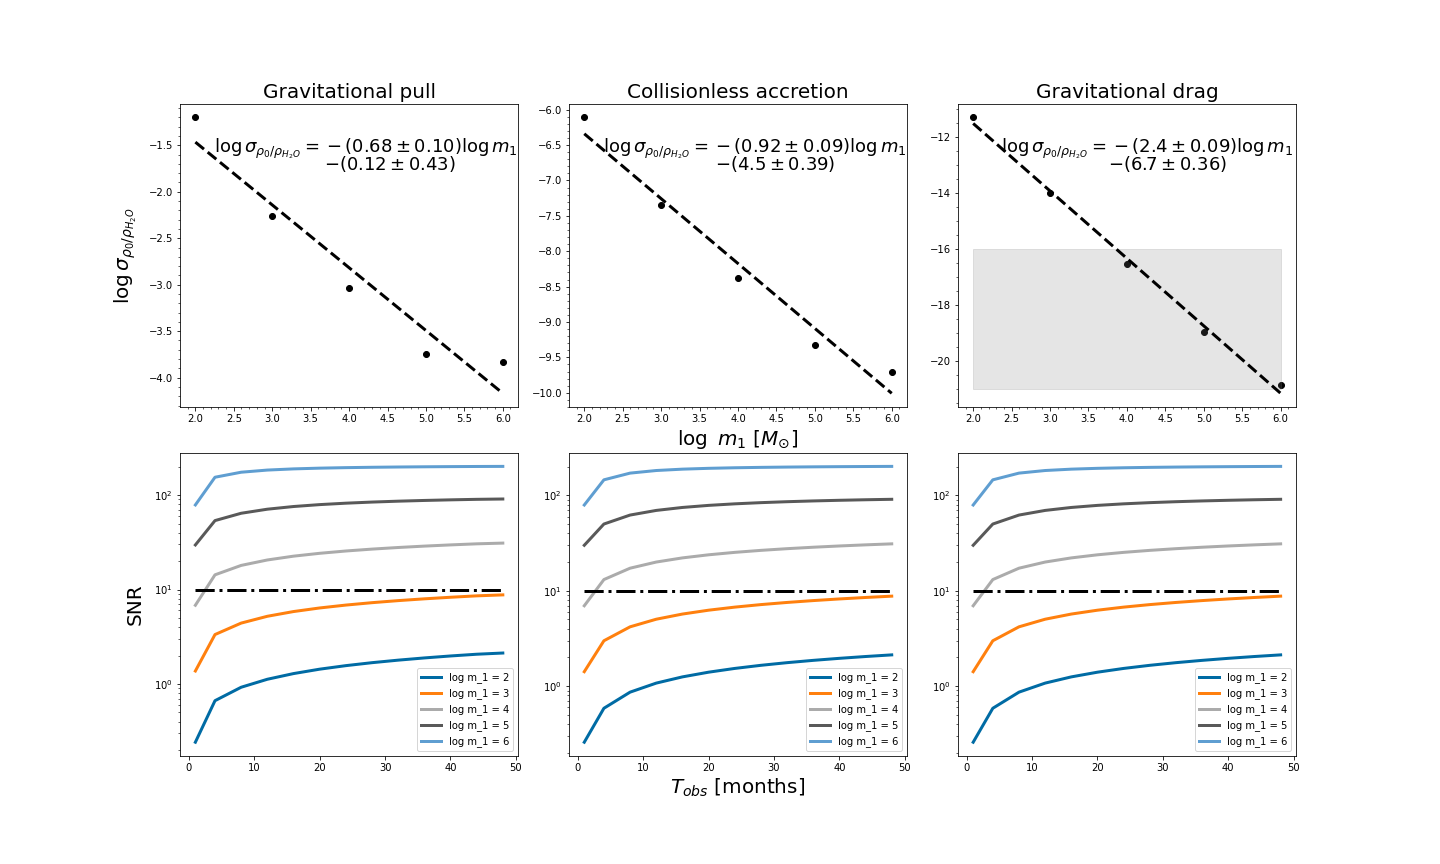
\includegraphics[width=\linewidth]{SPP2021_mainresults.png}
\caption{(Top row) 1-$\sigma$ uncertainties for the density of the surrounding medium (normalized to water density) as a function of the primary mass of the simulated binaries. The density range typical of accretion disks span $\rho_0/\rho_{\text{H}_2\text{O}} \in [10^{-16}, 10^{-1}]$, while the density range typical of dark matter span $\rho_0/\rho_{\text{H}_2\text{O}} \in [10^{-25}, 10^{-16}]$ (shaded gray region). Also shown are the best-fit log-log relationships (dashed lines). (Bottom row) Signal-to-noise ratio of the difference between the vacuum IMRPhenomB waveform and environmentally-modified waveform as a function of observation time for different primary masses. The modified waveforms used are for binaries living in $\rho_0 = 10^{3} ~\text{kg}/\text{m}^3$ environments. The dot-dash line indicates the conservative SNR estimate for signal detection.}
\label{fig:results}
\end{figure}

Table \ref{table:binaryparams} shows the source parameters $\mathcal{M}, ~\eta, ~\chi_{\text{eff}}$, $f_{\text{min}}$ and $f_{\text{max}}$, as well as the number of completed orbital cycles for five simulated binaries with primary masses $m_1 \in \{10^2, 10^3, 10^4, 10^5, 10^6\} ~M_{\odot}$. These values enter the waveform construction and overlap calculations. We note that the calculations fail for $m_1 \geq 10^7 ~M_{\odot}$ since the detectable waveform is already past the inspiral phase ($f_{\text{min}} > f_{\text{max}}$). We also note that Ajith et.~al's IMRPhenomB model is not calibrated for higher mass ratios, so it would be better to use more accurate frequency domain waveforms for EMRIs with higher $q$ \cite{Isoyama2020}. 


\begin{table}[bp!]
\centering % center-align tables within a column
\caption{Chirp mass $\mathcal{M}$, symmetric mass ratio $\eta$, effective spin $\chi_{\text{eff}}$, minimum and maximum frequencies for the overlap integrals, and the number of orbital cycles for five simulated binaries. For each primary mass, we set other source parameters constant: $m_2/M_{\odot} = 10$, $\chi_1 = 0.8$, and $\chi_2 = 0.5$. We adapt the notation $x(y) = x \times 10^y$.}\label{table:binaryparams}
\begin{tabular}{c| c c c c c c}
\toprule
$\log m_1/M_{\odot}$ & $\mathcal{M}/M_{\odot}$ & $\eta$ & $\chi_{\text{eff}}$ & $f_{\text{min}}$ [Hz] & $f_{\text{max}}$ [Hz] & no. of cycles \\
\midrule
$2.0$ & $2.46(1)$ & $8.26(-2)$ & $7.72(-1)$ & $1.87(-2)$ & $1.00(0)$ & $3.75(6)$ \\
$3.0$ & $6.30(1)$ & $9.80(-3)$ & $7.97(-1)$ & $1.04(-2)$ & $1.00(0)$ & $2.09(6)$ \\
$4.0$ & $1.58(2)$ & $9.98(-4)$ & $8.00(-1)$ & $5.85(-3)$ & $1.00(0)$ & $1.17(6)$ \\
$5.0$ & $3.98(2)$ & $9.99(-5)$ & $8.00(-1)$ & $3.29(-3)$ & $1.13(-1)$ & $6.58(5)$ \\
$6.0$ & $9.99(2)$ & $1.00(-5)$ & $8.00(-1)$ & $1.85(-3)$ & $1.13(-2)$ & $3.53(5)$ \\
\bottomrule
\end{tabular}
\end{table}


%\subsection{Fisher matrix analysis}
From the calculated covariance matrices, we obtained the uncertainties of the surrounding density $\sigma_{\rho_0}$ marginalized over the other waveform parameters. We plot the values of $\log$ $\sigma_{\rho_0}$ against $\log$ $m_1$ for the three environmental effects in the top row of Figure \ref{fig:results}. We find that the uncertainties in the density of the surrounding medium follow an inverse log-log relationship with the primary mass, with the following best-fit exponents for gravitational pull, collisionless accretion, and gravitational drag, respectively: $-0.68 \pm 0.10$, $-0.92 \pm 0.09$, and $-2.4 \pm 0.09$. These results partially define the structure of the complete 6-dimensional covariance ellipsoid spanning the waveform parameter space. We note that as expected for all environmental effects, we were able to recover Cardoso and Maselli's results for $m_1 = 10^4 ~M_{\odot}$ and $m_1 = 10^5 ~M_{\odot}$ \cite{Cardoso2020}. 

%While this is a very specific relationship (since not all IMRI/EMRIs may have the same spins), 

%We also compare the order-of-magnitude estimates to that of the typical reported values for the density of accretion disks and dark matter. With the most constraining environmental effect (gravitational drag), LISA is able to probe densities typical of dark matter (in agreement with Cardoso and Maselli's results). Thus, we can use confirmed LISA candidates to distinguish the astrophysical environment of EMRIs.

We see that for the same primary masses, different environmental effects lead to different magnitudes of $\sigma_{\rho_0}$. Gravitational drag leads to the tightest constraints, probing densities typical of dark matter for $m_1 \geq 10^4 ~M_{\odot}$ (in the shaded gray region of Figure \ref{fig:results}). At this point we emphasize that in our calculations, the different environmental effects were considered independent of one another. This may be different from the realistic astrophysical scenario in which all three (as well as other effects) come into play. 

%By combining and weighing environmental effects, we may produce better constraints on the surrounding density.



%\subsection{Overlap analysis}\label{rnd:overlap}
The SNR calculations indicate that for the higher primary masses $10^4-10^6 ~M_{\odot}$, the difference between a vacuum and dephased waveform would be (almost instantly) visible to LISA, as seen in the bottom row of Figure \ref{fig:results}. This means that using a vacuum waveform template to match a signal with environmental dephasing may hamper detection, in agreement with the findings of Kocsis et.~al \cite{Kocsis2011} for different waveform and dephasing models.

For the simulated IMRI binaries, on the other hand, dephased and vacuum waveforms cannot be distinguished from each other, even after four years of observation. For all environmental effects affecting the binary with $m_1 = 10^3 ~M_{\odot}$, we find that the SNR of the waveform difference reaches the threshold of detection towards the end of the 4-year observation period, so that the difference would be detectable for sources that are closer than our reference luminosity distance of 1 Gpc.

%We may be able to show the perturbation for the lower mass binaries by using other detectors or adjusting the other waveform parameters such as the distance of the binary from the detector $d_L$.

%It would then be necessary to employ other search methods if we want to scrutinize the environment around these kinds of binaries. It would also be instructive to check other dephasing models that may deviate from this calculation, in order to ensure that the parameter space is well mapped.

%\begin{table}[b]
%\centering % center-align tables within a column
%\caption{Slope $a$ and y-intercept $b$ values of the best-fit lines $\log \sigma_{\rho_0} = a \log m_1 + b$ for three environmental effects}\label{table:bestfitparams}
%\begin{tabular}{l l c c}
%\toprule
%\multicolumn{2}{c}{Environmental effect} & Mean & Standard deviation\\
%\midrule
%\multirow{2}{7em}{Gravitational pull} & $a$ & -0.6754 & 0.10203 \\
%& $b$ & -0.1159 & 0.43286 \\
%\hline
%\multirow{2}{7em}{Collisionless accretion} & $a$ & -0.9169 & 0.09075 \\
%& $b$ & -4.506 & 0.38501 \\
%\hline
%\multirow{2}{8em}{Gravitational drag} & $a$ & -2.414 & 0.0856 \\
%& $b$ & -6.684 & 0.3631 \\
%\bottomrule
%\end{tabular}
%\end{table}


\section{Conclusions and recommendations}
In this paper, we have shown how LISA can distinguish the environment around IMRI/EMRI binaries using Fisher matrix analysis and overlap analysis of dephased and vacuum waveforms. These calculations can be used as a starting point in mapping the confidence intervals around the waveforms' true parameters, towards getting better estimates of the binary's environmental and source parameters. 

%However, these uncertainties and overlap calculations depend heavily on the waveform and dephasing model used. 

For future work, we can check for trends on the other source parameters to complete the confidence intervals. We can also map the Fisher ellipsoid in the waveform parameter space to obtain better constraints and determine degeneracies among waveform parameters \cite{Ohme2013}. Other dephasing models for environmental effects such as those considered in \cite{Kocsis2011} may also be studied. Finally, the assumption on the structure of the surrounding medium can be relaxed and more generic density profiles such as dark matter distributions (which make the surrounding medium's effects depend on its distance from the central BH) \cite{Cardoso2020} may be further studied. 
%To improve and scrutinize the environmental searches for IMRIs, it might be better to use detectors spanning the dHz range \cite{sedda2020missing}. 

\section*{Acknowledgments}
The authors would like to acknowledge the helpful discussions and inputs from the following: Ian Vega, Adrian Villanueva, Bence Kocsis, Nico Yunes, and Abraham Loeb. The authors also acknowledge the use of code generously provided by Vitor Cardoso and Andrea Maselli.



% Please use the style file spp-bst.bst. If you wish to use BibTeX, kindly use us the filename bibfile.bib for your bib file.
\bibliographystyle{spp-bst}
\bibliography{bibfile}

\end{document}